% !TeX program = pdfLaTeX
\documentclass[12pt]{article}
\usepackage{amsmath}
\usepackage{graphicx,psfrag,epsf}
\usepackage{enumerate}
\usepackage{natbib}
\usepackage{textcomp}
\usepackage[hyphens]{url} % not crucial - just used below for the URL
\usepackage{hyperref}

%\pdfminorversion=4
% NOTE: To produce blinded version, replace "0" with "1" below.
\newcommand{\blind}{0}

% DON'T change margins - should be 1 inch all around.
\addtolength{\oddsidemargin}{-.5in}%
\addtolength{\evensidemargin}{-.5in}%
\addtolength{\textwidth}{1in}%
\addtolength{\textheight}{1.3in}%
\addtolength{\topmargin}{-.8in}%

%% load any required packages here



% tightlist command for lists without linebreak
\providecommand{\tightlist}{%
  \setlength{\itemsep}{0pt}\setlength{\parskip}{0pt}}

% From pandoc table feature
\usepackage{longtable,booktabs,array}
\usepackage{calc} % for calculating minipage widths
% Correct order of tables after \paragraph or \subparagraph
\usepackage{etoolbox}
\makeatletter
\patchcmd\longtable{\par}{\if@noskipsec\mbox{}\fi\par}{}{}
\makeatother
% Allow footnotes in longtable head/foot
\IfFileExists{footnotehyper.sty}{\usepackage{footnotehyper}}{\usepackage{footnote}}
\makesavenoteenv{longtable}



\begin{document}


\def\spacingset#1{\renewcommand{\baselinestretch}%
{#1}\small\normalsize} \spacingset{1}


%%%%%%%%%%%%%%%%%%%%%%%%%%%%%%%%%%%%%%%%%%%%%%%%%%%%%%%%%%%%%%%%%%%%%%%%%%%%%%

\if0\blind
{
  \title{\bf Modeling K-12 school shootings as a clustered point process and an areal process, from 1990-2019}

  \author{
        J Steven Raquel \\
    Department of Statistics, University of California, Irvine\\
      }
  \maketitle
} \fi

\if1\blind
{
  \bigskip
  \bigskip
  \bigskip
  \begin{center}
    {\LARGE\bf Modeling K-12 school shootings as a clustered point process and an areal process, from 1990-2019}
  \end{center}
  \medskip
} \fi

\bigskip
\begin{abstract}

\end{abstract}

\noindent%
{\it Keywords:} 
\vfill

\newpage
\spacingset{1.45} % DON'T change the spacing!

\hypertarget{background}{%
\section{Background}\label{background}}

The prevalence of gun violence in schools in the United States has been referred to both as an ``epidemic'' and a public health crisis, and one that has steadily increased over the past several decades (see Figure \ref{fig:ts-plot-1990-2019}). The debate on how to curb these tragedies is a solidly partisan issue, with calls for more and stronger gun control laws, as well as more mental health care, sometimes as an alternative to gun control. Concealed carry laws are argued both in favor of, and against and are labeled as both an enabler and a potential deterrent to mass shootings. Apart from the trauma that such an event can bring to a community, there is also resonant fear that such incidents inspire ``copycat'' events on a local and a larger scale. This spatial analysis attempts to model the incidence of these shootings as a Poisson point process, in order to ascertain whether the locations and events occur with complete spatial randomness. We also model the data in an areal form on a per-state basis so as to compare it against the level of gun control and mental health care, also on a state level.

\hypertarget{data}{%
\subsection{Data}\label{data}}

The school shooting data was sourced directly from the ``K-12 School Shooting Database'' made available by the Center for Homeland Defense and Security (CHDS). The information that comprises the dataset was determined by a specific process which entailed asking what exactly comprises a school shooting. Most shootings that were premeditated and resulted in mass casualties, such as those that occurred at Columbine in 1999, Sandy Hook in 2012, and Stoneman Douglas in 2018, are considered ``indiscriminate shootings''. Although the original database contains shootings ruled accidental (from misuse of a firearm) as well as incidences of gang-related gun violence on school grounds, among other incidents, we did not opt to consider this data as relevant to this study in particular.

\begin{figure}
\centering
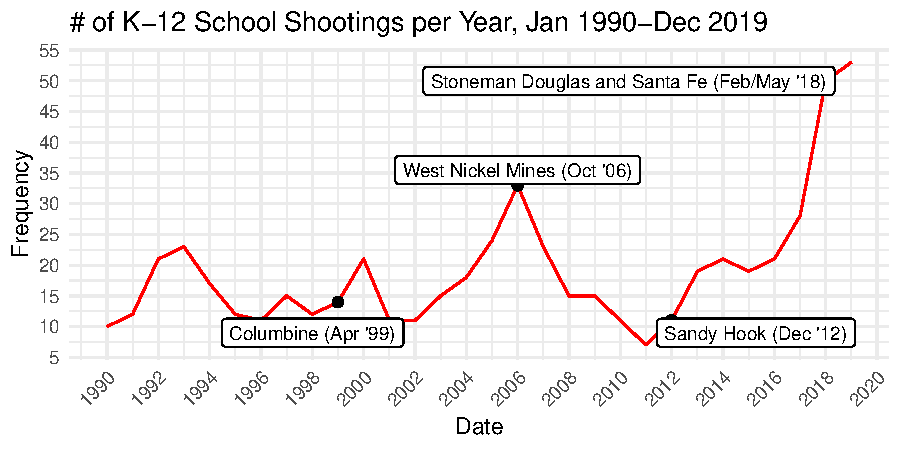
\includegraphics{JStevenRaquel_STATS295_Final_files/figure-latex/ts-plot-1990-2019-1.pdf}
\caption{\label{fig:ts-plot-1990-2019}Time series plot of number of K-12 school shootings per year, from Jan 1990 to Dec 2019.}
\end{figure}

It was a deliberate decision on our part to filter out these incidents as others like it so as to hone in one the more specific and cultural recognized definition of a school shooting, which is an attack that takes place on school grounds, in order to target students, faculty, or passersby with the intent to cause terror and/or inflict harm on specific individuals. Targeted events related to domestic situations (e.g.~anger over a break-up), or the escalation of disputes (e.g.~fistfights in which one person pulls out a firearm) were also ruled school shootings.

The database originally goes as far back as 1970 all the way to present day (March 2022 at the time of this writing), but it was of particular interest to look at the data after 1990 since this consolidates the modern era in which access to firearms and the incidence of gun violence in schools is more normalized. It was also decided to leave out data past 2019 as the COVID-19 pandemic which hit the US in 2020 is a huge confounding variable as it caused many schools to institute remote learning which decreased the incidence of shootings on school campuses.

The data originally only contained the name of the school, as well as the city and state where the events took place, but we were able to use the Google Maps API to source the specific latitude/longitude coordinates of these events.

In addition to this school shooting data, we also have gun control data consisting of several columns of binary categorical data as to whether or not a certain law (e.g.~a ban on concealed carry, background checks) is instituted in a given state for the years between 1991 and 2020 from StateFirearmLaws.org, as well as mental healthcare data from 2019 courtesy of Mental Health America (MHA), which consists of a ranking of all 50 states and the District of Columbia on their ratio of need for and accessibility to mental healthcare. More information on these resources can be found on their respective websites (see References section).

\hypertarget{methods}{%
\section{Methods}\label{methods}}

\hypertarget{exploratory-data-analysis}{%
\subsection{Exploratory Data Analysis}\label{exploratory-data-analysis}}

As a preliminary analysis, we chose to plot this data on both a point and at an areal level, for a number of reasons. For one, modeling the data as a point pattern allows us to test the null hypothesis for complete spatial randomness against the alternative hypothesis of clustering. It allows us to hone in on exactly where within a given state might be considered a ``hotspot'' for a shooting. Conversely, the areal data allows us to compare the number of incidents in a given state and look at it with respect to the level of gun control and mental healthcare available there as well.

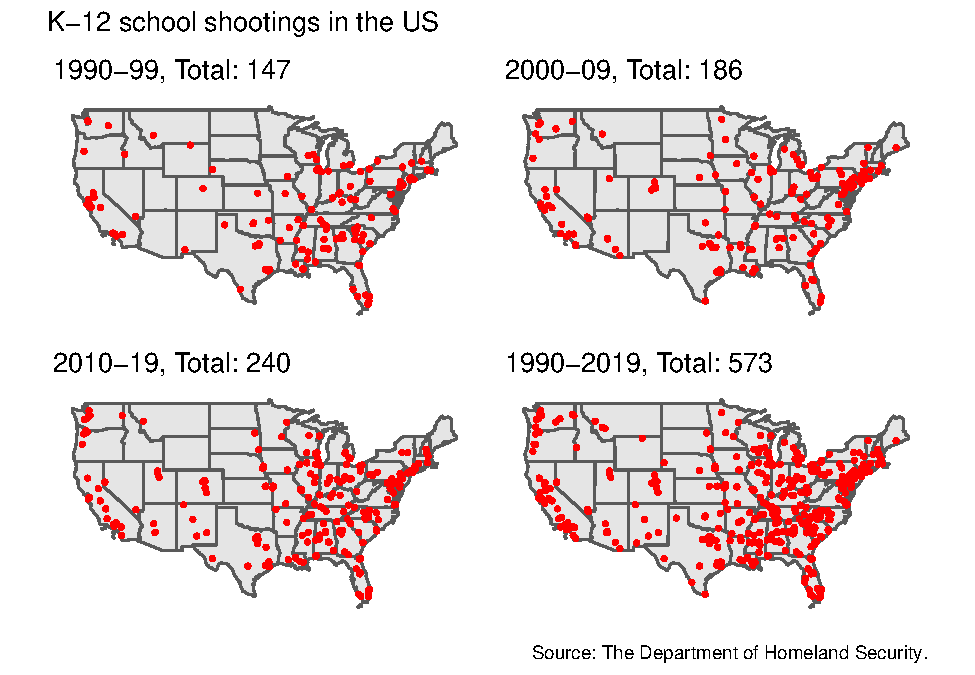
\includegraphics{JStevenRaquel_STATS295_Final_files/figure-latex/plots-all-four-1.pdf}

As we can see from the

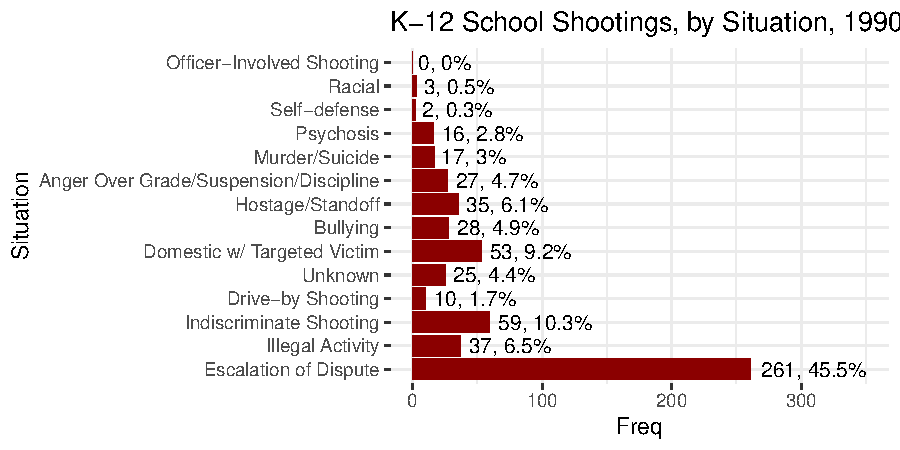
\includegraphics{JStevenRaquel_STATS295_Final_files/figure-latex/plot-situation-1.pdf}

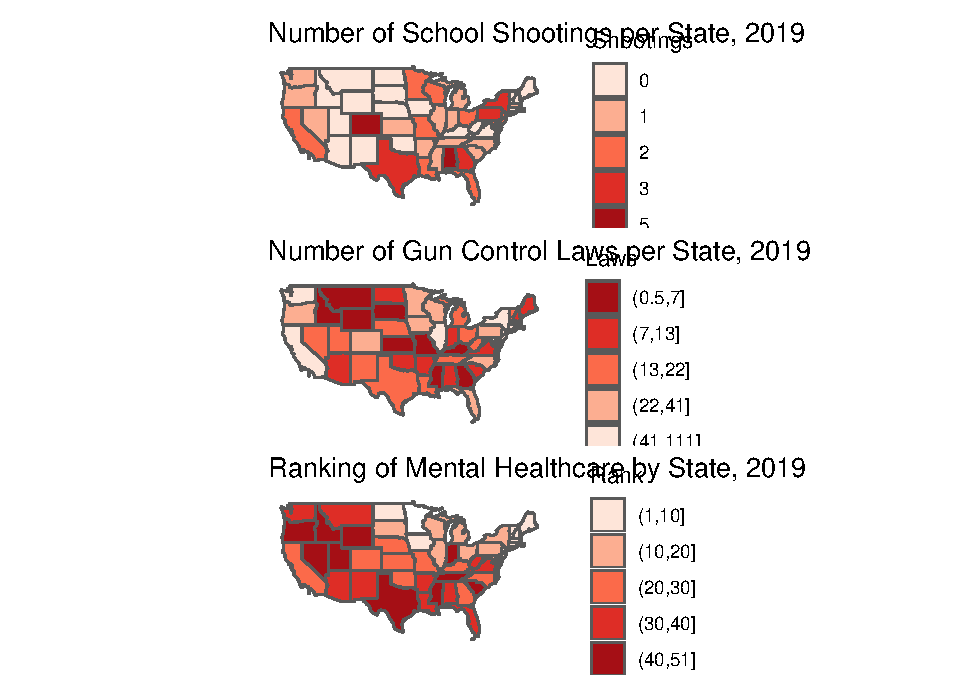
\includegraphics{JStevenRaquel_STATS295_Final_files/figure-latex/plot-areals-2019-1.pdf}

\hypertarget{point-pattern-analysis}{%
\subsection{Point Pattern Analysis}\label{point-pattern-analysis}}

As with any spatial point pattern analysis, we are concerned with the following three questions, 1) whether the points are located at random, 2) whether they are clustered, and 3) whether they are placed regularly. The hypothesis of \emph{complete spatial randomness} (CSR) asserts the following:

\begin{itemize}
\tightlist
\item
  The number of events in any region \(S\) with area \(|S|\) follows a Poisson distribution with mean \(\lambda |S|\), where \(\lambda\) is the intensity, i.e.~\(\lambda\) does not change over \(S\)
\item
  Given \(n\) events in \(S\), the points \(s_i\) are independently located according to the uniform distribution on \(S\), i.e.~there is no interaction amongst events.
\end{itemize}

The intensity function \(\lambda(s)\), also known as the first-order property of the spatial point process, is defined as

\[\lambda(s) = \lim_{|\Delta s| \to 0} \frac{E[N(\Delta s)]}{| \Delta s|}\]

Firstly we want to ascertain whether the incidences of school shootings are indeed a Poisson process, and if so, determine whether or not the process is \emph{homogeneous} (where the intensity function \(\lambda(s)\) assumes a constant \(\lambda\)) or \emph{inhomogeneous}. Contextually, this means we are interested in ascertaining whether the spatial pattern of these shootings is random or not, i.e.~are they more likely to take place in certain places, or around each other? The intensity function is the expected number of events per unit area.

\hypertarget{quadrats}{%
\subsection{Quadrats}\label{quadrats}}

While we could estimate the intensity function across the entire area, what we are interested in this particular analysis is to how the intensity varies across different regions contained therein. We do this by splitting up the area into what are referred to as \emph{quadrats}.

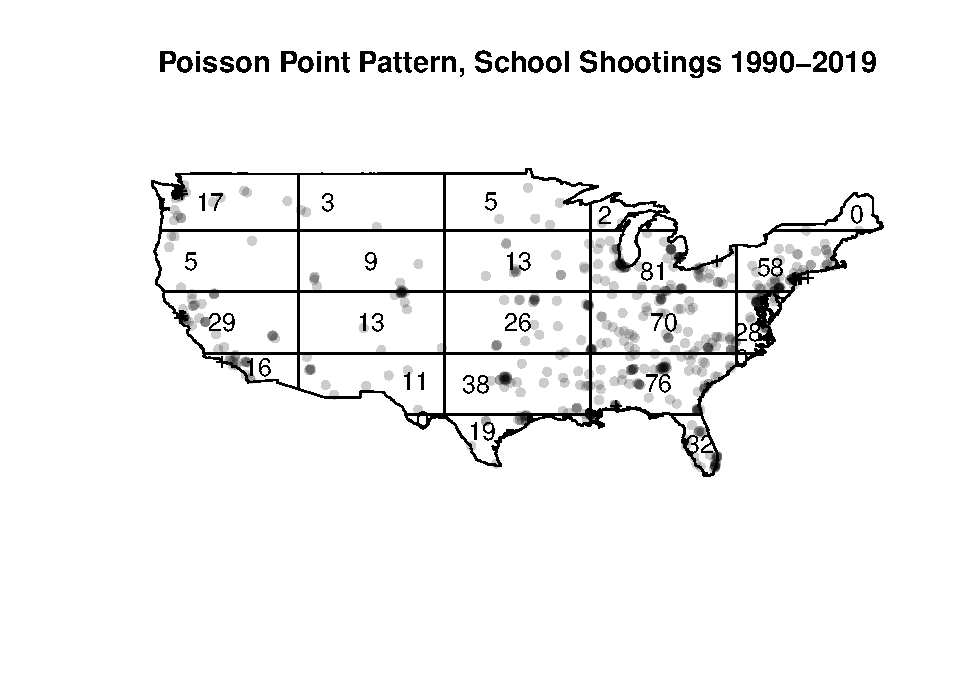
\includegraphics{JStevenRaquel_STATS295_Final_files/figure-latex/plot-ppp-1990-2019-1.pdf}

\begin{verbatim}
## 
##  Conditional Monte Carlo test of CSR using quadrat counts
##  Test statistic: Pearson X2 statistic
## 
## data:  ppp_9019
## X2 = 582.1, p-value = 2e-04
## alternative hypothesis: clustered
## 
## Quadrats: 23 tiles (irregular windows)
\end{verbatim}

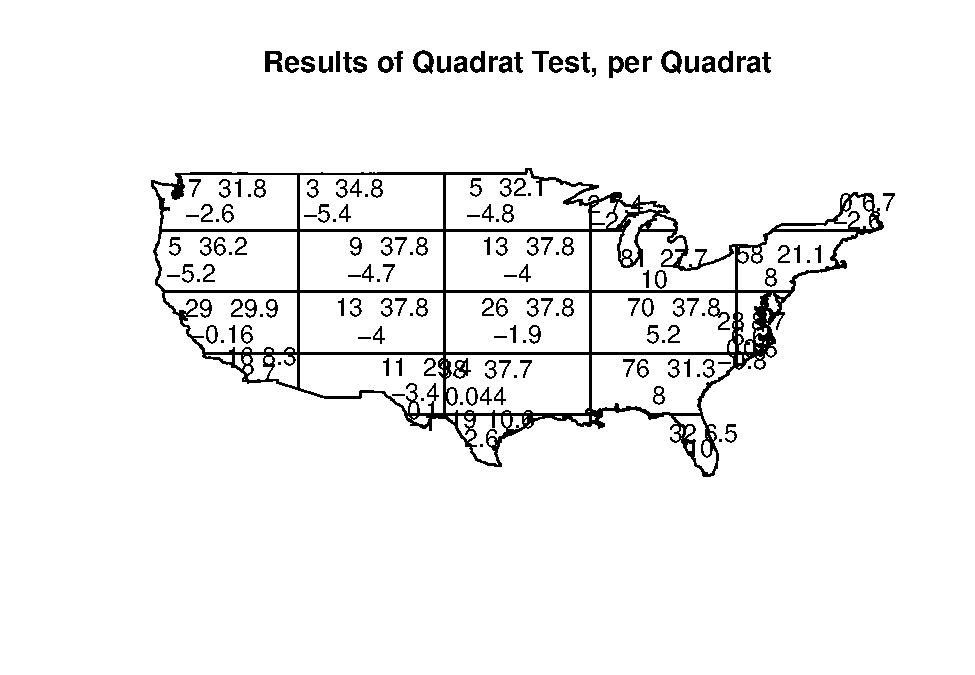
\includegraphics{JStevenRaquel_STATS295_Final_files/figure-latex/quadrat-test-1.pdf}
\#\# Kernel Density

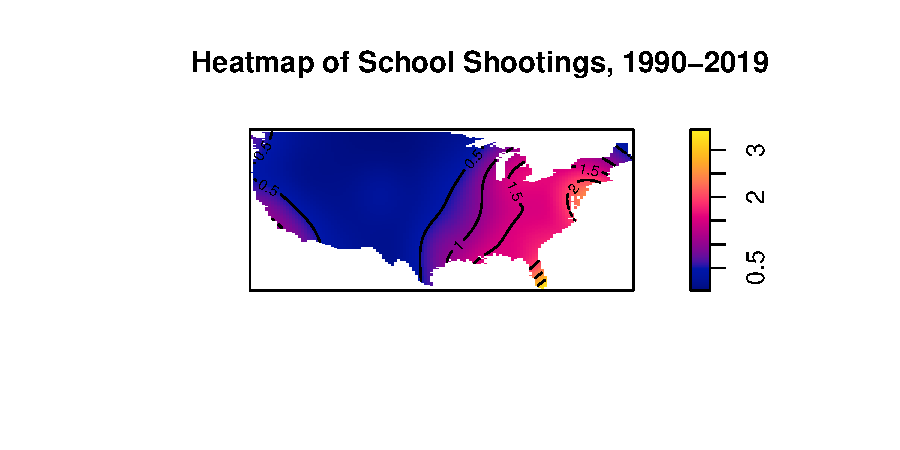
\includegraphics{JStevenRaquel_STATS295_Final_files/figure-latex/density-90-19-1.pdf}

\hypertarget{nearest-neighbor}{%
\subsection{Nearest Neighbor}\label{nearest-neighbor}}

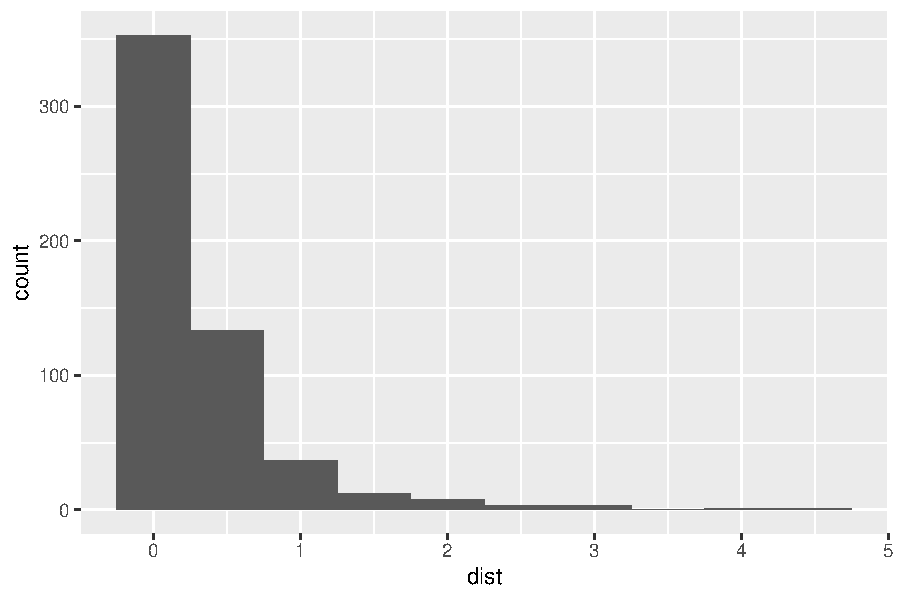
\includegraphics{JStevenRaquel_STATS295_Final_files/figure-latex/nearest-neighbor-1.pdf}

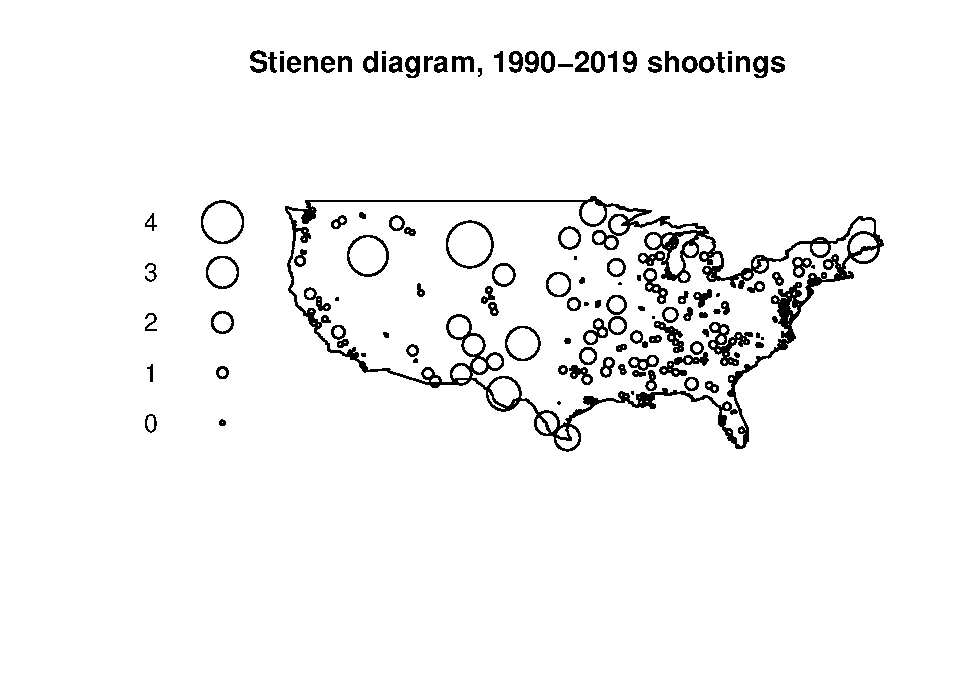
\includegraphics{JStevenRaquel_STATS295_Final_files/figure-latex/Sienen-diagram-1.pdf}

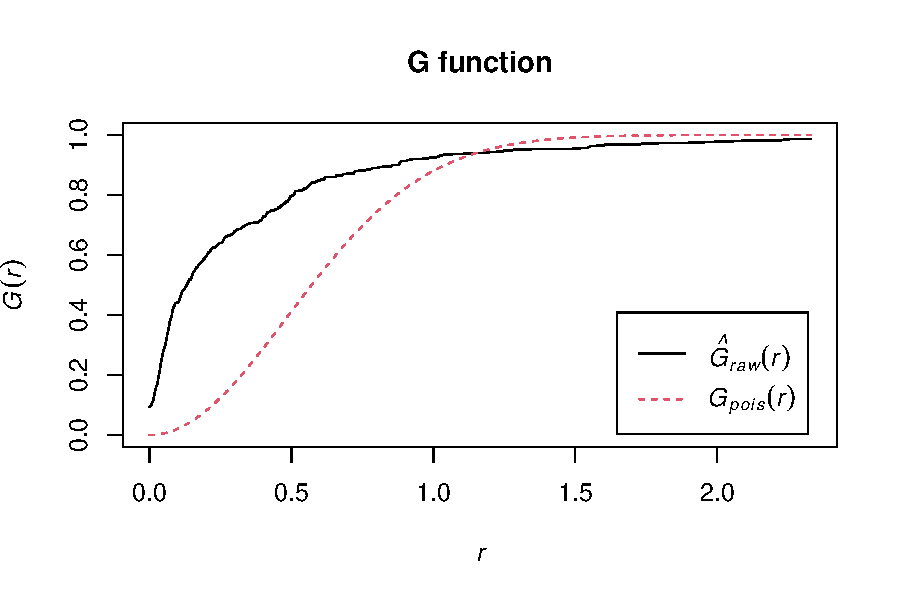
\includegraphics{JStevenRaquel_STATS295_Final_files/figure-latex/G-function-1.pdf}

\hypertarget{discussion}{%
\section{Discussion}\label{discussion}}

\hypertarget{references}{%
\section{References}\label{references}}

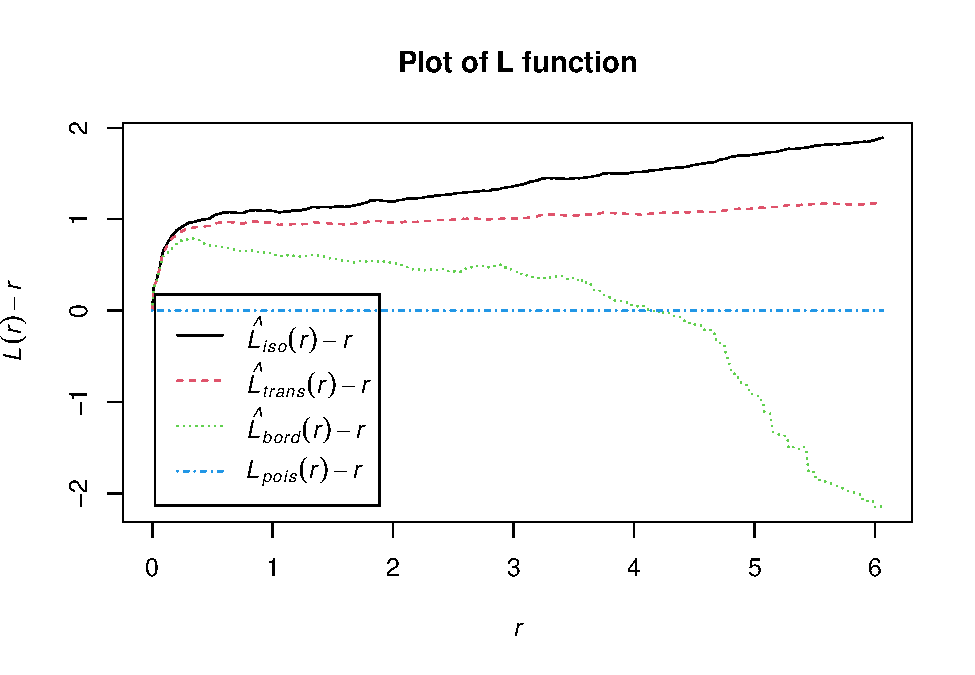
\includegraphics{JStevenRaquel_STATS295_Final_files/figure-latex/KL-functions-1.pdf}

\newpage

\hypertarget{references-1}{%
\section{References}\label{references-1}}

\newpage

\bibliographystyle{agsm}
\bibliography{}


\end{document}
